\documentclass[11pt, oneside]{article}   	% use "amsart" instead of "article" for AMSLaTeX format
\usepackage[margin=1in]{geometry}                		% See geometry.pdf to learn the layout options. There are lots.
\geometry{letterpaper}                   		% ... or a4paper or a5paper or ... 
%\geometry{landscape}                		% Activate for rotated page geometry
%\usepackage[parfill]{parskip}    		% Activate to begin paragraphs with an empty line rather than an indent
\usepackage{graphicx}				% Use pdf, png, jpg, or eps§ with pdflatex; use eps in DVI mode
								% TeX will automatically convert eps --> pdf in pdflatex		
\usepackage{amssymb}
\usepackage{awesomebox}
%SetFonts

%SetFonts

\usepackage{amsmath}
%\DeclareMathOperator{\mod}{mod}
\let\emptyset\varnothing

\newcommand{\reals}{\mathbb{R}}
\newcommand{\realsText}{$\mathbb{R}$}
\newcommand{\ints}{\mathbb{Z}}
\newcommand{\intsText}{$\mathbb{Z}$}

\title{Homework 3}
\author{Discrete Structures 1}
\date{due: 7 March 2023, 8:00am}							% Activate to display a given date or no date

\begin{document}
\maketitle
%\section{}
%\subsection{}

Your task for this homework will be to answer the following questions without using any calculating resources. 
Your responses should be submitted via blackboard by the due date above as a PDF (submissions in any other format will be returned to the user and a resubmissions will be requested). 
You are free to use whatever tools you would like to generate the response document: 
scanned hand-written paper, 
tablet generated hand-written, 
microsoft word (with this option, please use the equation editor to correctly format your responses), 
\LaTeX, etc.
Your TA, IA, and Instructor are available to help during their designated office hours or via email 
(note that emails sent during non-business hours may not be responded to until the next working day). 

%\importantbox{
%\textbf{Note:} all of these questions are on topics from chapters 5; thus you will only be proving by induction in this homework assignment. 
%}
\begin{enumerate}
% 3.1
\item What is the truth values of the following propositions: 22 + 32 = 42
% 3.13 
\item The identity of a binary operator $\diamond$ is a value $i$ such that, for any $x$, the expressions \\$\{x,x\diamond i,i\diamond x\}$ are all equivalent.
An example from arithmetic: 
the identity of $+$ is $0$, because $x + 0 = 0 + x = x$ for any number $x$. 
\begin{enumerate}
\item Identify the identity of $\vee$, and justify your answer. (Some operators do not have an identity; if there is no identity, explain why it doesn’t exist.)
\item What is the identity of $\wedge$? (Or, if it doesn’t exist, explain why not.)
\item What is the identity of $\leftrightarrow$? (Or, if it doesn’t exist, explain why not.)
\item What is the identity of $\oplus$? (Or, if it doesn’t exist, explain why not.)
\end{enumerate}
\item \label{question:binary}
In addition to purely logical operations, computer circuitry has to be built to do simple arithmetic very quickly. 
Consider a number $x \in {0, . . . , 15}$ represented as a 4-bit binary number, 
and denote by $x_0$ the least-significant bit of $x$, by $x_1$ the next bit, and so forth. 
(Think of 0 as false and 1 as true.) 
Here you’ll explore some pieces of using propositional logic and binary representation of integers to express arithmetic operations. 
(It’s straightforward to convert your answers into circuits.) 
See Figure~\ref{fig:binary}.
\begin{enumerate}
%3.28
\item Give a proposition over $\{x_0 , x_1 , x_2 , x_3 \}$ that expresses that $x$ is greater than or equal to 8.
%3.29
\item Give a proposition over $\{x_0 , x_1 , x_2 , x_3 \}$ that expresses that $x$ is evenly divisible by 4.
%3.31
\item Give a proposition over $\{x_0 , x_1 , x_2 , x_3 \}$ that expresses that $x$ is evenly divisible by 9.
\tipbox{ you may want to make a truth table}
\end{enumerate}
\begin{figure}
\centering
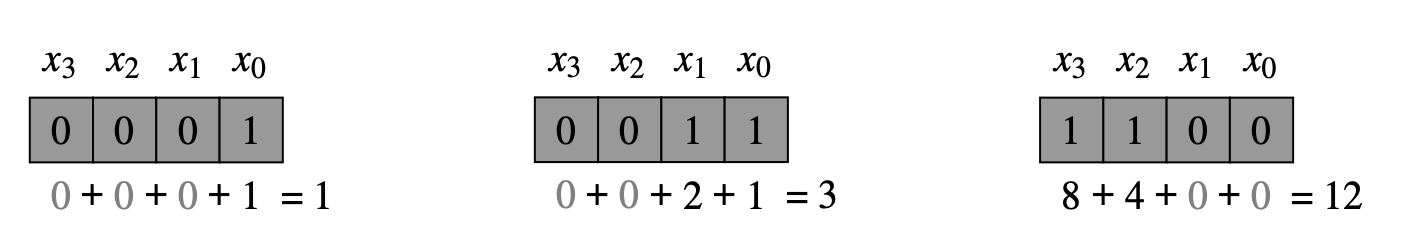
\includegraphics[width=0.75\textwidth]{small_binary}
\caption{Some examples for Question~\ref{question:binary}}
\label{fig:binary}
\end{figure}

\end{enumerate}
\end{document}